\chapter*{Введение}                         % Заголовок
\addcontentsline{toc}{chapter}{Введение}    % Добавляем его в оглавление

\newcounter{XXcnt}
\setcounter{XXcnt}{20}

Параллельные и распределённые вычисления -- сравнительно новая область, бурно развивающаяся с середины \Roman{XXcnt} века\cite{FirstComputers} и продолжающая существенный рост до сих пор. В последнее время этот рост подстёгивается развитием специализированных устройств, таких как видеокарты, специализированные платы для машинного обучения и ускорители для других выделенных задач. Такие устройства часто не предусматривают возможности запуска операционной системы и прямого взаимодействия с пользователем. Вместо этого они полагаются на то, что где-то существует обычный компьютер, играющий роль \textbf{хоста} который подготавливает вычислительные задачи или \textbf{оффлоады} и отправляет их на устройства, которые заточены на решение задач такого рода.

Такой подход называется гетерогенными вычислениями \cite{shan2006heterogeneous}, так как роли хоста и устройства или устройств не равны и они не взаимозаменяемы. Поскольку современные видеокарточки это программируемые процессоры, по мощности часто превосходящие управляющую машину, критичным становится вопрос выбора программного интерфейса между хостом и устройствами. Исторически существует много программных интерфейсов (API) разного качества и с разными целями, как открытых так и закрытых, специфичных для конкретного производителя \cite{HeteroSurvey}.

\begin{figure}[ht]
    \centerfloat{
        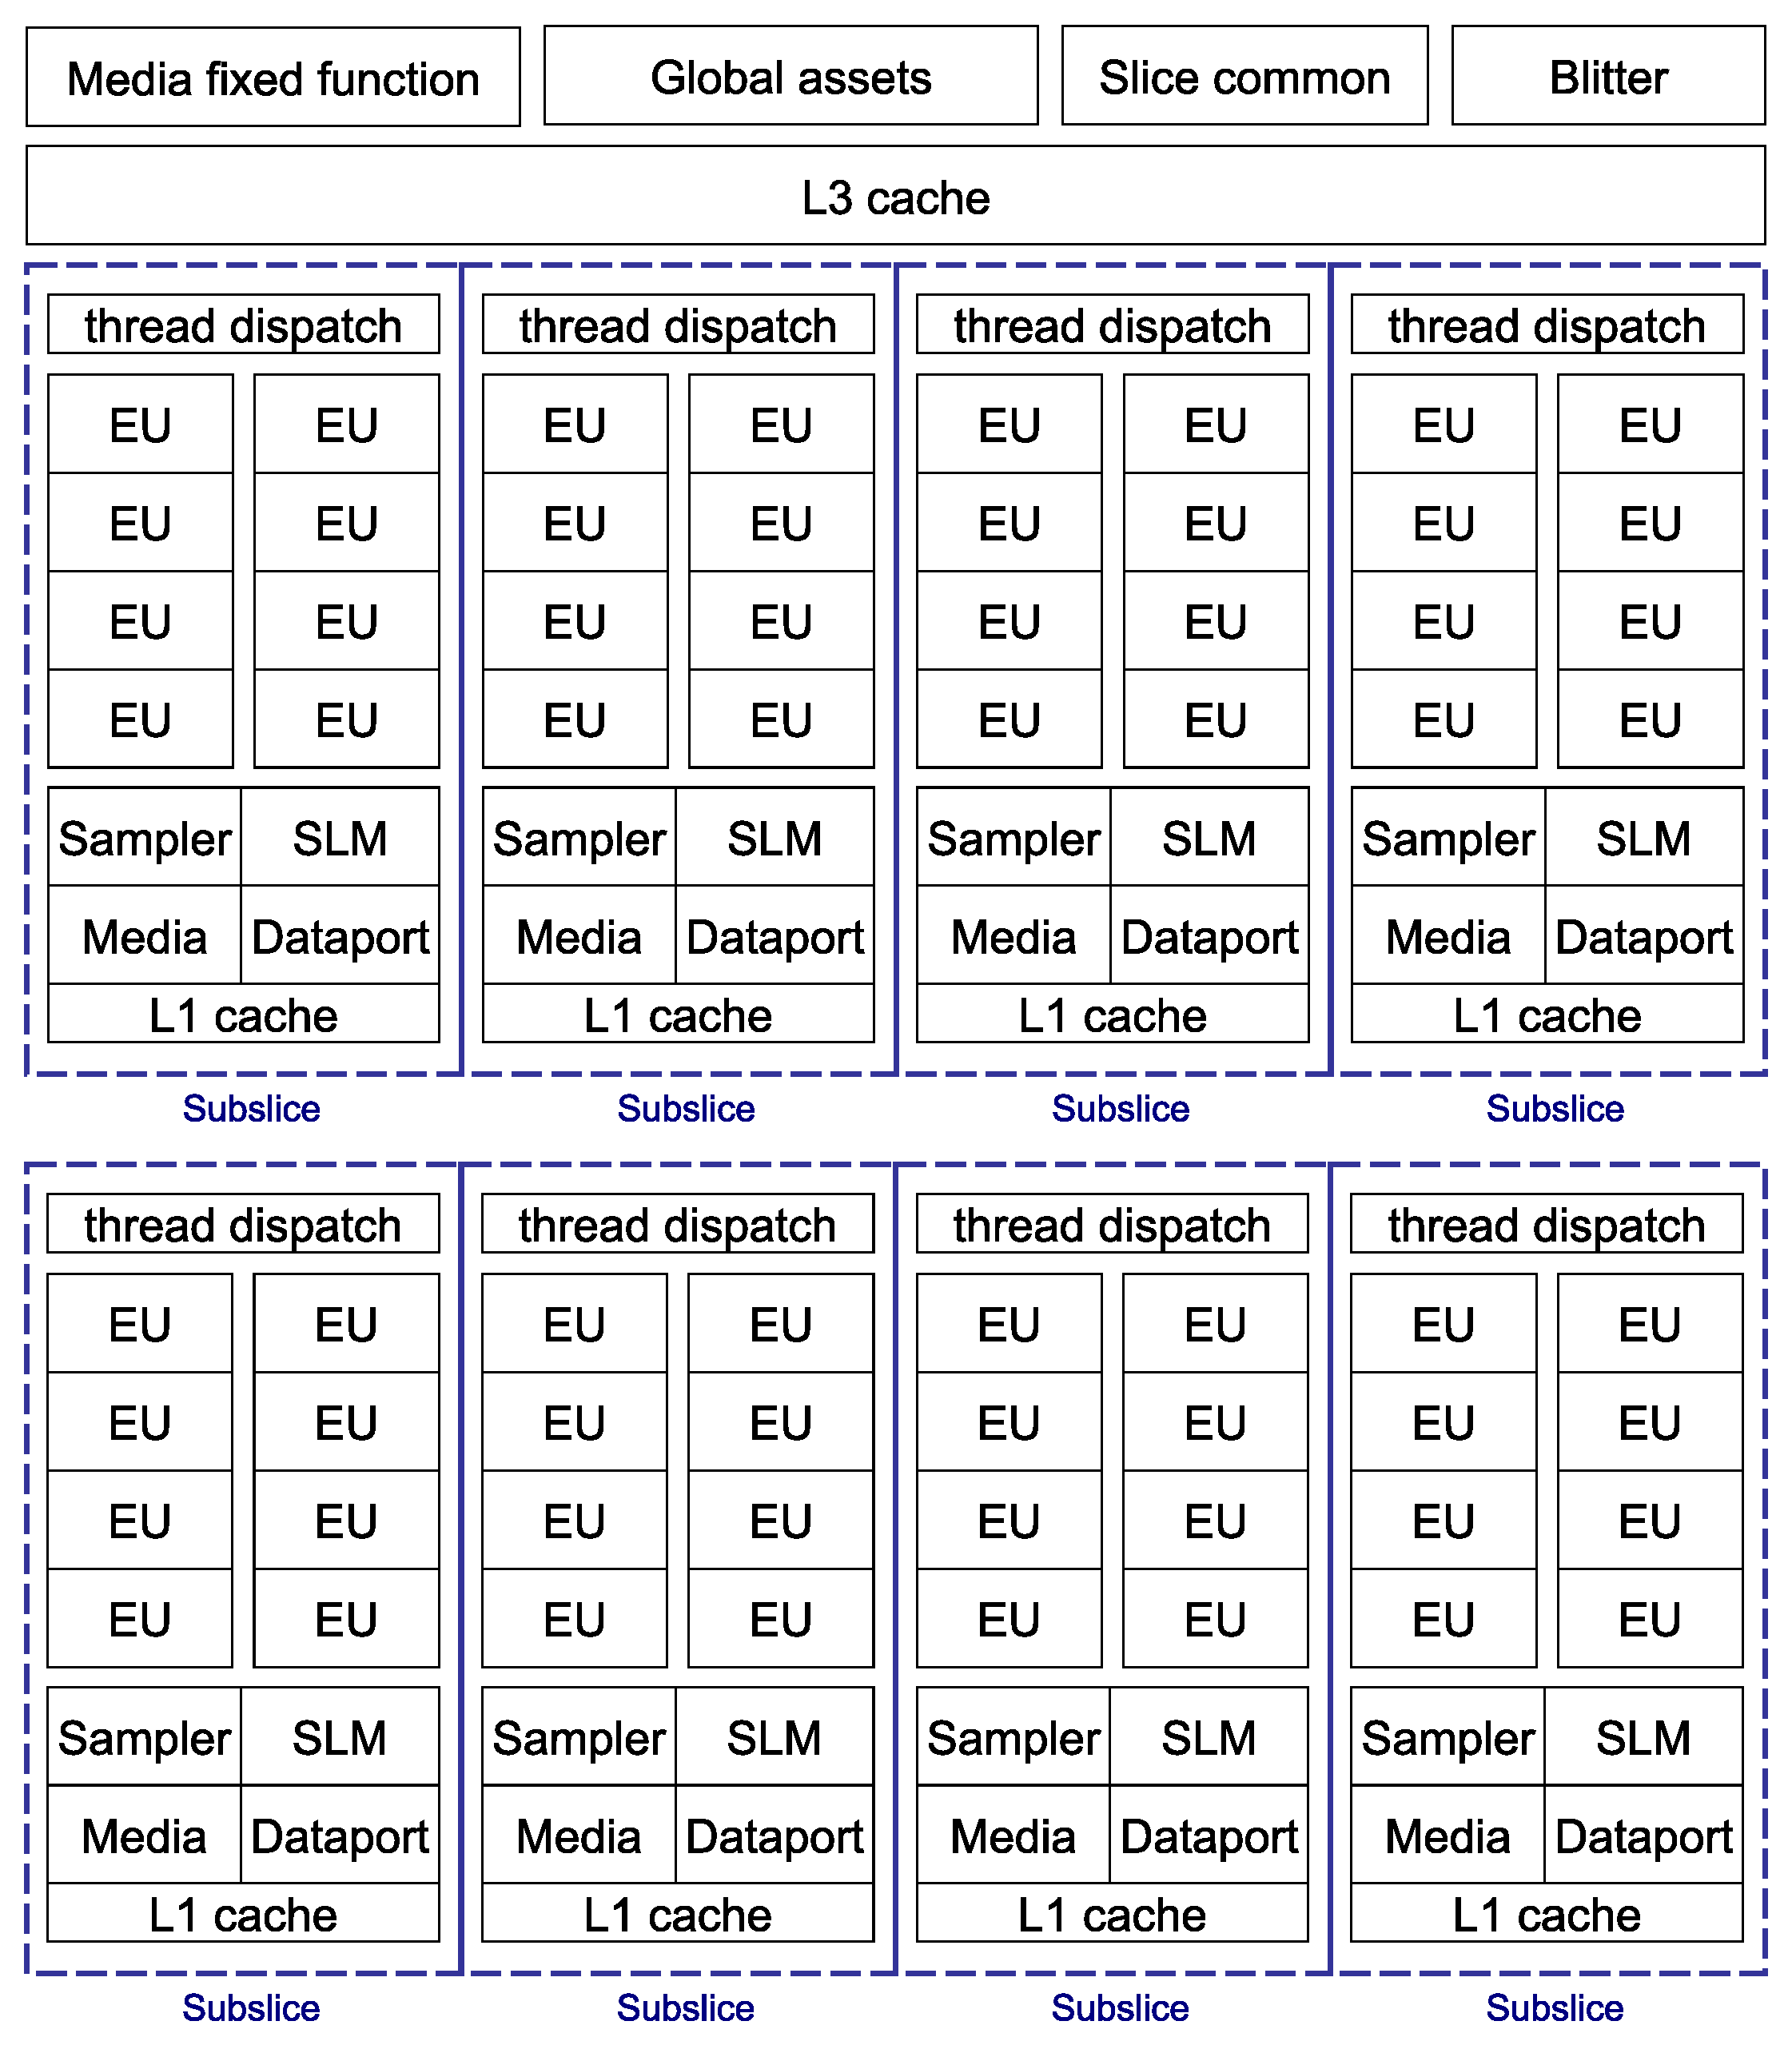
\includegraphics[scale=0.4]{Vladimirov/images/typical-GPU.pdf}
    }
    \caption{Типичное устройство GPU на примере Intel Gen 11}\label{fig:typicalGPU}
\end{figure}

Типичная современная видеокарточка (вариант Intel Gen 11) представлена на рисунке~\cref{fig:typicalGPU}. Можно видеть большое количество параллельных исполнительных устройств, у каждого из которых есть небольшой кеш первого уровня и на всех один общий кеш третьего уровня (второй уровень пропущен конструктивно). Также в каждом подслое (subslice) можно увидеть блок локальной памяти (SLM), порт для общения с глобальной памятью и некоторые фиксированные функции (медиаблок, самплер).
\nomenclature{\(SLM\)}{shared local memory, разделяемая локальная память}
\nomenclature{\(CPU\)}{central processing unit, центральный процессор}
\nomenclature{\(GPU\)}{graphics processing unit, видеокарточка}
\nomenclature{\(NPU\)}{neural processing unit, карта машинного обучения}
\nomenclature{\(API\)}{neural processing unit, карта машинного обучения}

С развитием оыбчных процессоров (CPU), количество ядер на них увеличивается. Обычно для функций контроля устройств и подготовки вычислительных задач нужно не более одного аппаратного потока. Это приводит к тому, что гетерогенная система может быть построена не только из специализированных устройств но и из свободных от функций хоста ядер хостового процессора. Такой подход называется гибридным программированием \cite{yang2017hybrid}. При таком подходе можно пересылать данные в глобальную видеопамять и инициировать гетерогенные вычисления через один интерфейс (например CUDA), а потоками хостовой машины управлять через другой интерфейс (например OpenMP). Это возможный подход к гибридной системе но конечно гораздо лучше когда вычислительная задача может быть исполнена на самых разных устройствах и все доступные устройства объединены единым интерфейсом.

На такой единый открытый интерфейс претендует, например, SYCL \cite{da2016comparative}. Есть также вариант SYCL с расширениями Intel, который называется DPC++ \cite{reinders2021dpc}. Но использование таких программных интерфейсов предполагает работу с логической моделью памяти. И здесь критически важной становится то, насколько хорошо мы оптимизируем одну и ту же программу для работы с совершенно разными устройствами. Разумеется каждое устройство имеет собственный компилятор. Например для видеоускорителей компании Intel компилятор называется Intel Graphics Compiler и он доступен публично \cite{chandrasekhar2019igc}.

Таким образом тема исследований оптимизаций в компиляторах для гетерогенных программ и в частности для графических ускорителей является актуальной. Первые публикации по этой теме начали появляться в 2000-х годах \cite{yang2010gpgpu} и тема сравнительно хорошо разработана для скалярных программных интерфейсов, например для уже упоминавшегося OpenMP \cite{lee2009openmp}. Тема которая почти не освещена в текущей литературе это работа с векторными системами команд и оптимизации памяти и потока управления для векторных программных интерфейсов. Эта работа во многом мотивирована появлением высокоуровневых векторных программных интерфейсов, таких как DPC++ESIMD и ISPC \cite{pharr2012ispc}. Язык и система программирования ISPC отлично показали себя на задачах трассировки лучей на векторных CPU, таких как процессоры Intel с расширениями AVX. Необходимость переноса этого успеха на гетерогенные и гибридные системы ставит задачу компиляции высокоуровневого векторного представления в векторную систему команд. Эта задача частично решалась графическим компилятором Intel, но как оптимальность так и функциональная корректность решения оставляли простор для исследований, особенно в части работы с памятью. Так например ранние попытки компилировать программы на ISPC для GPU показали внезапно худшую производительность чем на CPU. Эта работа адресует многие из возникших проблем и является результатом более чем трёхлетней работы автора в компании Intel и преподавания в МФТИ.

\textbf{Целью} данной работы является разработка методов и алгоритмов оптимизации работы с памятью в гетерогенных системах.

Для~достижения поставленной цели необходимо было решить следующие \textbf{задачи}:
\begin{enumerate}[beginpenalty=10000] % https://tex.stackexchange.com/a/476052/104425
  \item Разработать методологию представления высокоуровневых векторных конструкций в векторной системе команд.
  \item Разработать алгоритм разбиения структур данных для улучшения векторизации.
  \item Разработать алгоритм восстановления векторного потока управления.
\end{enumerate}

\iffalse

% TODO: такая структура это хорошая идея но мне пока не хочется портить common

\newcommand{\actuality}{}
\newcommand{\progress}{}
\newcommand{\aim}{{\textbf\aimTXT}}
\newcommand{\tasks}{\textbf{\tasksTXT}}
\newcommand{\novelty}{\textbf{\noveltyTXT}}
\newcommand{\influence}{\textbf{\influenceTXT}}
\newcommand{\methods}{\textbf{\methodsTXT}}
\newcommand{\defpositions}{\textbf{\defpositionsTXT}}
\newcommand{\reliability}{\textbf{\reliabilityTXT}}
\newcommand{\probation}{\textbf{\probationTXT}}
\newcommand{\contribution}{\textbf{\contributionTXT}}
\newcommand{\publications}{\textbf{\publicationsTXT}}

\newcommand{\actuality}{\pdfbookmark[1]{Актуальность}{actuality}\underline{\textbf{\actualityTXT}}}
\newcommand{\progress}{\pdfbookmark[1]{Разработанность темы}{progress}\underline{\textbf{\progressTXT}}}
\newcommand{\aim}{\pdfbookmark[1]{Цели}{aim}\underline{{\textbf\aimTXT}}}
\newcommand{\tasks}{\pdfbookmark[1]{Задачи}{tasks}\underline{\textbf{\tasksTXT}}}
\newcommand{\aimtasks}{\pdfbookmark[1]{Цели и задачи}{aimtasks}\aimtasksTXT}
\newcommand{\novelty}{\pdfbookmark[1]{Научная новизна}{novelty}\underline{\textbf{\noveltyTXT}}}
\newcommand{\influence}{\pdfbookmark[1]{Практическая значимость}{influence}\underline{\textbf{\influenceTXT}}}
\newcommand{\methods}{\pdfbookmark[1]{Методология и методы исследования}{methods}\underline{\textbf{\methodsTXT}}}
\newcommand{\defpositions}{\pdfbookmark[1]{Положения, выносимые на защиту}{defpositions}\underline{\textbf{\defpositionsTXT}}}
\newcommand{\reliability}{\pdfbookmark[1]{Достоверность}{reliability}\underline{\textbf{\reliabilityTXT}}}
\newcommand{\probation}{\pdfbookmark[1]{Апробация}{probation}\underline{\textbf{\probationTXT}}}
\newcommand{\contribution}{\pdfbookmark[1]{Личный вклад}{contribution}\underline{\textbf{\contributionTXT}}}
\newcommand{\publications}{\pdfbookmark[1]{Публикации}{publications}\underline{\textbf{\publicationsTXT}}}


\input{common/characteristic} % Характеристика работы по структуре во введении и в автореферате не отличается (ГОСТ Р 7.0.11, пункты 5.3.1 и 9.2.1), потому её загружаем из одного и того же внешнего файла, предварительно задав форму выделения некоторым параметрам

\textbf{Объем и структура работы.} Диссертация состоит из~введения,
\formbytotal{totalchapter}{глав}{ы}{}{},
заключения и
\formbytotal{totalappendix}{приложен}{ия}{ий}{}.
%% на случай ошибок оставляю исходный кусок на месте, закомментированным
%Полный объём диссертации составляет  \ref*{TotPages}~страницу
%с~\totalfigures{}~рисунками и~\totaltables{}~таблицами. Список литературы
%содержит \total{citenum}~наименований.
%
Полный объём диссертации составляет
\formbytotal{TotPages}{страниц}{у}{ы}{}, включая
\formbytotal{totalcount@figure}{рисун}{ок}{ка}{ков} и
\formbytotal{totalcount@table}{таблиц}{у}{ы}{}.
Список литературы содержит
\formbytotal{citenum}{наименован}{ие}{ия}{ий}.
\fi